\documentclass[a4paper, 12pt]{article}
\usepackage{geometry}
\geometry{a4paper,
total={170mm,257mm},left=2cm,right=2cm,
top=2cm,bottom=2cm}

\usepackage{mathtext}
\usepackage{amsmath}
\usepackage[utf8]{inputenc}
\usepackage[english,russian]{babel}
\usepackage{graphicx, float}
\usepackage{tabularx, colortbl}
\usepackage{caption}
\captionsetup{labelsep=period}

\newcommand{\parag}[1]{\paragraph*{#1:}}
\DeclareSymbolFont{T2Aletters}{T2A}{cmr}{m}{it}
\newcounter{Points}
\setcounter{Points}{1}
\newcommand{\point}{\arabic{Points}. \addtocounter{Points}{1}}
\newcolumntype{C}{>{\centering\arraybackslash}X}

\author{Калинин Даниил, Б01-110}
\date{\today}
\title{Лабораторная работа 2.1.3.\\Определение $\frac{C_p}{C_v}$ через измерение скорости звука}

\begin{document}
\maketitle

\parag {Цель работы} измеренить частоты колебаний и длины волны при резонансе звуковых колебаний в газе, заполняющем трубу; определенить показатель адиабаты с помощью уравнения состояния идеального газа.

\parag {В работе используются}
звуковой генератор ГЗ; электронный осциллограф ЭО; микрофон; телефон; теплоизолированная труба, обогреваемая водой из термостата.

\parag {Теоритическая справка} ~\\
Скорость распространения звуковой волны в газах зависит от показателя адиабаты $ \gamma $. Один из наиболее точных методов определения показателя адиабаты основан на измерении скорости звука.
    
Скорость звука в газах определяется формулой:
    
\begin{equation}
    \label{speed_of_sound}
    c=\sqrt{\gamma\frac{RT}{\mu}}
\end{equation}

где $ R $ -- газовая постоянная, $ T $ -- температура газа, а $ \mu $ -- его молярная масса. Преобразуя эту формулу, найдем

\begin{equation}
    \label{gamma}
    \gamma = \frac{c^2 \mu}{RT}
\end{equation}
    
Таким образом, для определения показателя адиабаты достаточно измерить температуру газа и скорость распространения звука (молярная масса газа предполагается известной).
    
Звуковая волна, распространяющаяся вдоль трубы, испытывает многократные отражения от торцов. Звуковые колебания в трубе являются наложением всех отраженных волн и очень сложны. Картина упрощается, если длина трубы $L$ равна целому числу полуволн, то есть когда \[L=n \frac{\lambda}{2}\] где $\lambda$ -- длина волны звука в трубе, а $n$ -- любое целое число. Если это условие выполнено, то волна, отраженная от торца трубы, вернувшаяся к ее началу и вновь отраженная, совпадает по фазе с падающей. При этом мплитуда звуковых колебаний при этом резко возрастает -- наступает резонанс.
    
При звуковых колебаниях слои газа, прилегающие к торцам трубы, не испытывают смещения. Узлы смещения повторяются по всей длине трубы через $\frac{\lambda}{2}$. Между узлами находятся максимумы смещения.
    
Скорость звука c связана с его частотой $\nu$ и длиной волны $ \lambda $ соотношением
    
\begin{equation}
    \label{lambda_nu}
    c=\lambda \nu
\end{equation}
    
Будем плавно изменять частоту колебаний $\nu$ звукового генератора, пока не заметим резкое увеличение амплитуды (резонанс) на осциллографе. Тогда, для последовательных резонансов, получим:

\begin{equation}
    \label{resonances}
    L=\frac{\lambda_1}{2}n = \frac{\lambda_2}{2}\left(n+1\right) = \dots = \frac{\lambda_{k+1}}{2}\left(n+k\right).
\end{equation}

Таким образом, из \eqref{lambda_nu} и \eqref{resonances} имеем:

\begin{equation}
    \label{nu}
    \nu_{k+1} = \frac{c}{\lambda_{k+1}} = \frac{c}{2L}\left(n+k\right)= \nu_1 + \frac{c}{2L} k
\end{equation}

То есть величина $\dfrac{c}{2L}$, определяется по угловому коэффициенту графика зависимости частоты $\nu$ от номера резонанса $k$.

\parag {Экспериментальная установка} ~\\

    
В работе используется установка (рис. \ref{setup}). Данная установка содержит теплоизолированную трубу постоянной длины. Воздух в трубе нагревается водой из термостата. Температура газа принимается равной температуре омывающей трубу воды. 

Звуковые колебания в трубе возбуждаются телефоном Т и улавливаются микрофоном М. Мембрана телефона приводится в движение переменным током звуковой частоты; в качестве источника переменной ЭДС используется звуковой генератор ГЗ. Возникающий в микрофоне сигнал наблюдается на осциллографе ЭО.

Микрофон и телефон присоединены к установке через тонкие резиновые трубки. Такая связь достаточна для возбуждения и обнаружения звуковых колебаний в трубе и в то же время мало возмущает эти колебания: при расчетах оба торца трубы можно считать неподвижными, а влиянием соединительных отверстий пренебречь.

\begin{figure}[H]
    \centering
    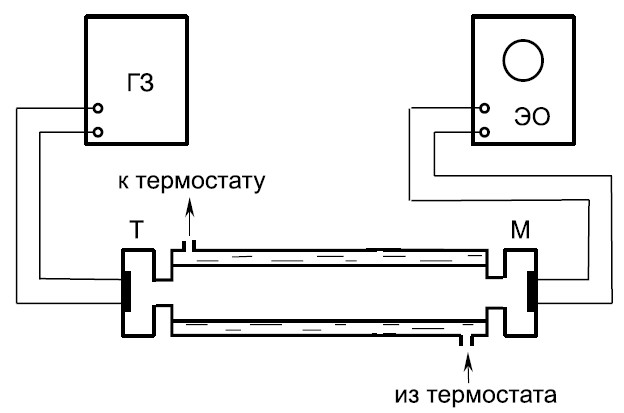
\includegraphics[width=10cm]{setup.jpg}
    \caption{\textit{Установка, на которой проводился эксперимент}}
    \label{setup}
\end{figure}

\parag {Ход работы} ~\\
\point Снимем комнатную температуру и длину трубы. Результат занесем в таблицу \ref{tabl:initails}.

\begin{table}[h]
    \centering
    \begin{tabular}{|l|l|}
    \hline 
    Величина                        & Значение          \\ \hline
    Длина трубы, $L$                & $700 \pm 1$ мм.   \\ \hline
    Комнатная температра, $T_к$     & $22.6^{\circ} C$  \\ \hline
    \end{tabular}
	\caption{Данные измерения комнатной температуры и длины трубы}
    \label{tabl:initails}
\end{table}

\point Запустим ЭО и ГЗ, проводим начальную настройку осциллографа, выбираем нужный режим (синусоидальный) на ГЗ.

\point Подбирем частоту на ГЗ таким образом, чтобы амплитуда резонансных колебаний на ЭО была достаточно велика.

\point Медленно увеличиваем частоту колебаний на ГЗ, записываем резонансные частоты. Повторяем эксперимент для различных температур от комнатной ($T_к = 22.6^{\circ} C$, до $T = 50^{\circ} C$). Данные заносим в таблицу \ref{tabl:data}.

\begin{table}[h]
    \centering
    \begin{tabular}{|c|c|c|c|c|c|c|}
    \hline 
    Номер резонанса ($k$)   & \multicolumn{6}{|c|}{Температура, $^\circ C$} \\ \hline
                            & $22.6^{\circ} C$ & $30^{\circ} C$ & $35.4^{\circ} C$ & $45^{\circ} C$ & $47.5^{\circ} C$ & $50^{\circ} C$  \\ \hline

    1	&	 497	&	 500	&	 506	&	 520	&	 525	&	 528	\\ \hline
    2	&	 750	&	 742	&	 754	&	 770	&	 780	&	 780	\\ \hline
    3	&	 992	&	1000	&	1010	&	1030	&	1031	&	1032	\\ \hline
    4	&	1230	&	1250	&	1257	&	1270	&	1280	&	1283	\\ \hline
    5	&	1478	&	1490	&	1520	&	1520	&	1535	&	1542	\\ \hline
    6	&	1720	&	1740	&	1756	&	1780	&	1785	&	1800	\\ \hline
                            
    \end{tabular}
	\caption{Резонансные частоты, в зависимости от температуры газа, Гц.}
    \label{tabl:data}
\end{table}

\point Отметим результаты на графике следующим образом: по оси абцисс будем откладывать номер резонанса $k$, а по оси ординат -- разность $\nu_{k + 1}$ и $\nu_1$-й частот. Для каждой из температур построим такую зависимость. Графики полученных зависимостей изображены на рисунках \ref{fig:freqs_to_resonances} и \ref{fig:freqs_to_resonances_in_diff_plots}.

\begin{figure}[hb]
    \centering
    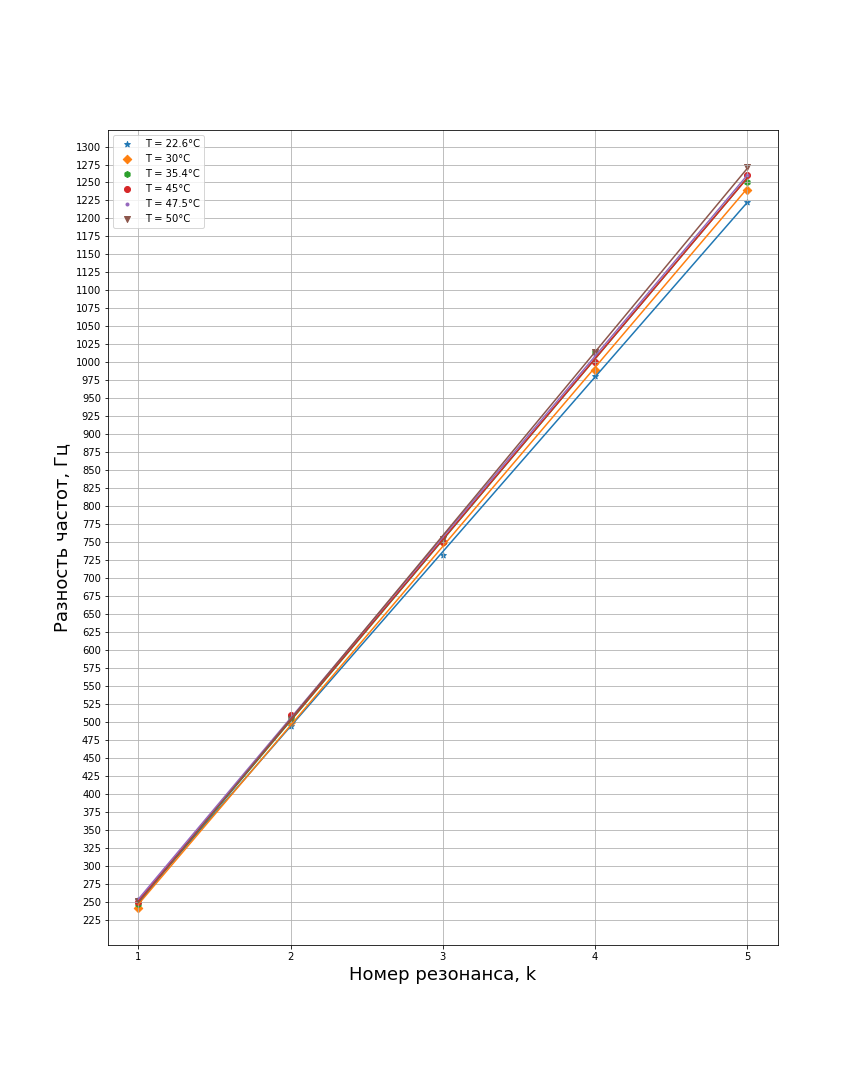
\includegraphics[width=0.7\linewidth]{freqs_to_resonances.png}
    \caption{\textit{График зависимости $\nu_{k + 1}$ и $\nu_1$ частот от номера резонанса $k$ для всех температур.}}
    \label{freqs_to_resonances}
\end{figure}

\begin{figure}[hb]
    \centering
    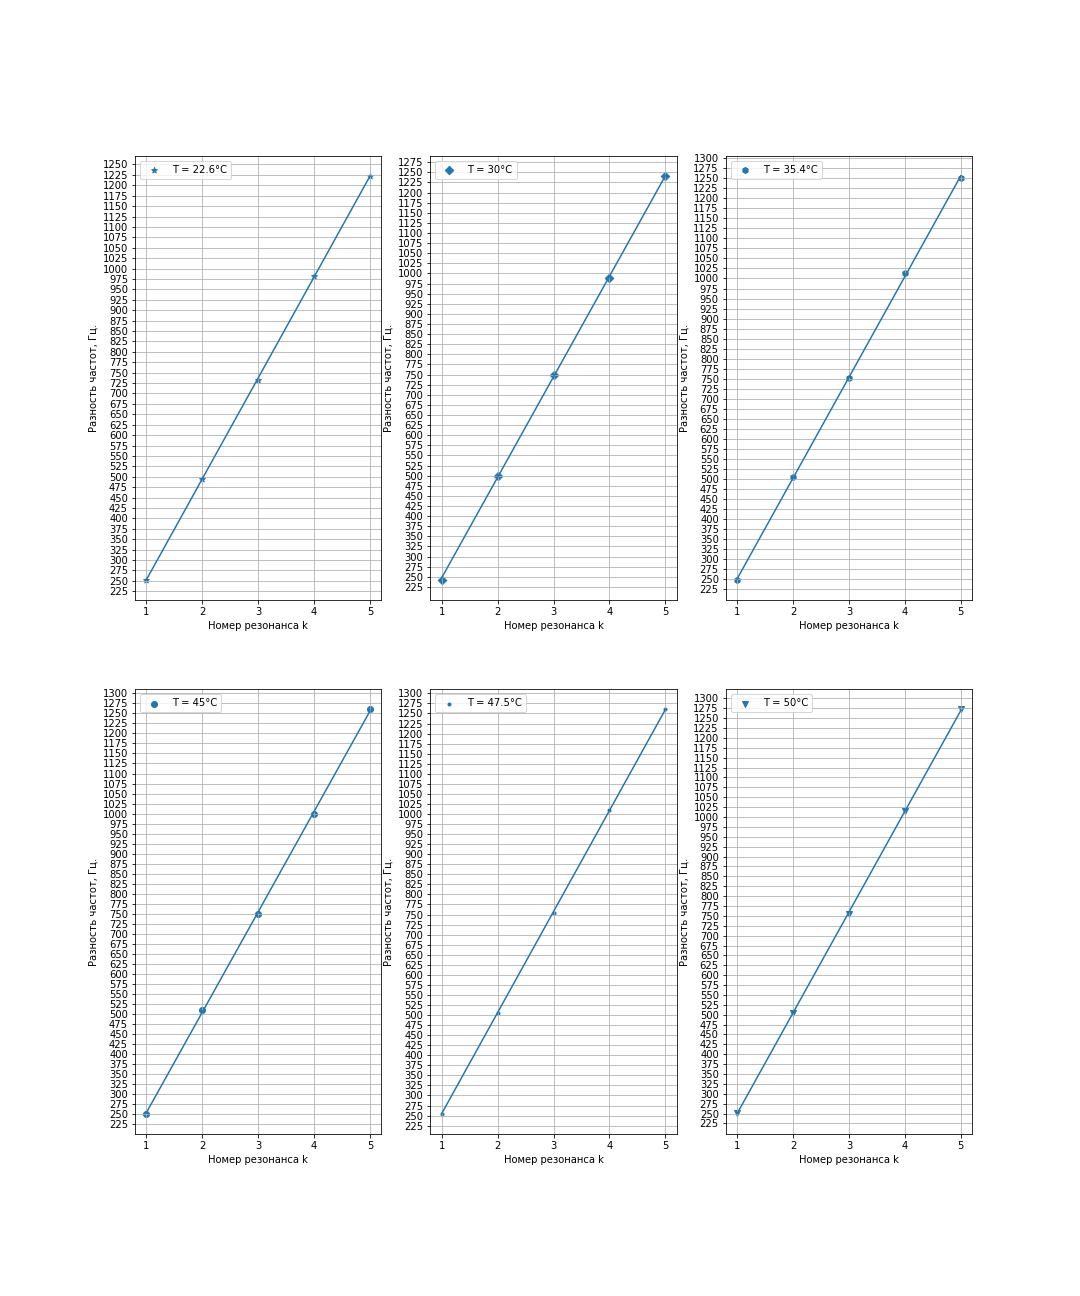
\includegraphics[width=0.7\linewidth]{freqs_to_resonances_in_diff_plots.png}
    \caption{\textit{График зависимости $\nu_{k + 1}$ и $\nu_1$ частот от номера резонанса $k$ для каждой температуры отдельно.}}
    \label{freqs_to_resonances_in_diff_plots}
\end{figure}

\point Посчитаем коэффициенты построенных прямых и погрешности их вычисления, результаты приведем в таблице \ref{tabl:line_coefs}.


\begin{table}[h]
    \centering
    \small
    \setlength\tabcolsep{3pt}

    \begin{tabular}{|c|c|c|c|c|c|c|c|}
    \hline 
    Температура, $^\circ C$ & $22.6$ & $30.0$ & $35.4$ & $45.0$ & $47.5$ & $50.0$ \\ \hline

    $с / \left(2 L\right),~ c^{-1}$ & $242.60 \pm 0.40$ & $248.60 \pm 0.84$ & $251.40 \pm 1.06$ & $251.00 \pm 0.94$ & $251.40 \pm 0.24$ & $255.00 \pm 0.52$ \\ \hline
    \end{tabular}
	\caption{Коэффициенты построенных прямых и погрешности их вычисления}
    \label{tabl:line_coefs}
\end{table}

\point По формуле \ref{gamma} вычислим показатели адиабаты для каждой температуры (принимая $\mu_{воздуха} = 28.98~\left(\frac{грамм}{моль}\right), R = 8.31~\left(\frac{Дж}{К \cdot моль}\right)$). Результаты занесем в таблицу \ref{tabl:gammas}

\begin{table}[h]
    \centering
    \small
    \setlength\tabcolsep{3pt}
    \begin{tabular}{|c|c|c|c|c|c|c|c|}
    \hline 
    Температура, $^\circ C$ & $22.6$ & $30.0$ & $35.4$ & $45.0$ & $47.5$ & $50.0$ \\ \hline
    Показатель адиабаты $\gamma$, & $1.3596$ & $1.3928$ & $1.3994$ & $1.3529$ & $1.3466$ & $1.3747$ \\ \hline
    Погрешность, & $\pm 0.0042$ & $\pm 0.0067$ & $\pm 0.0079$ & $\pm 0.0070$ & $\pm 0.0032$ & $\pm 0.0047$ \\ \hline
    \end{tabular}
	\caption{Коэффициенты построенных прямых и погрешности их вычисления}
    \label{tabl:gammas}
\end{table}

\point Усредняя вычисленные значения, получим:

$$\gamma = 1.3710 \pm 0.0056$$
$$\varepsilon = 4.1 \cdot 10^{-3} \approx 0.4\%$$

\parag {Заключение} ~\\
    В ходе данной работы был расчитан показатель адиабаты $\gamma$. Помимо того, было определено, что с высокой точностью можно считать, что показатель адиабаты не зависит от температуры газа в диапазоне температур от $T_{min} = 20^circ C$ до $T_{max} = 50^\circ C$. Была проверена зависимость скорости звука в воздухе от температуры. Полученные результаты можно улучшить, увеличив точность измерения резонансных частот. Тем не менее, относительная ошибка в $0.4\%$ это неплохой результат.
\end{document}
